% intro
In this section a background on the theory involved in Bayesian Coevluation. It is divided into neural networks, gaussian processes and (co)evolution. Neural networks are shortly described as they are used them for policy representation. Gaussian processes is a key concept in our approach to maintain a believe over the fitness of policies and evolution is used as a means to do policy search. First, however, a definition for rare controllable events is provided.

\subsection{Rare controllable events}
Figure %\ref{rareControllableImage} 
shows the rareness of an event and the performance of two policies on those events. Rare events are those of which the chance of occurring is very small, while controllability is defined as the influence of an agent is on the reward in that event. An event where there exists a policy that perform much better than an other policy is an event where the policy has a high influence on (with respect to the reward), and thus controllable. A rare controllable event is then an event which is both rare and controllable.

% \begin{figure}[h]
%   \centering
%   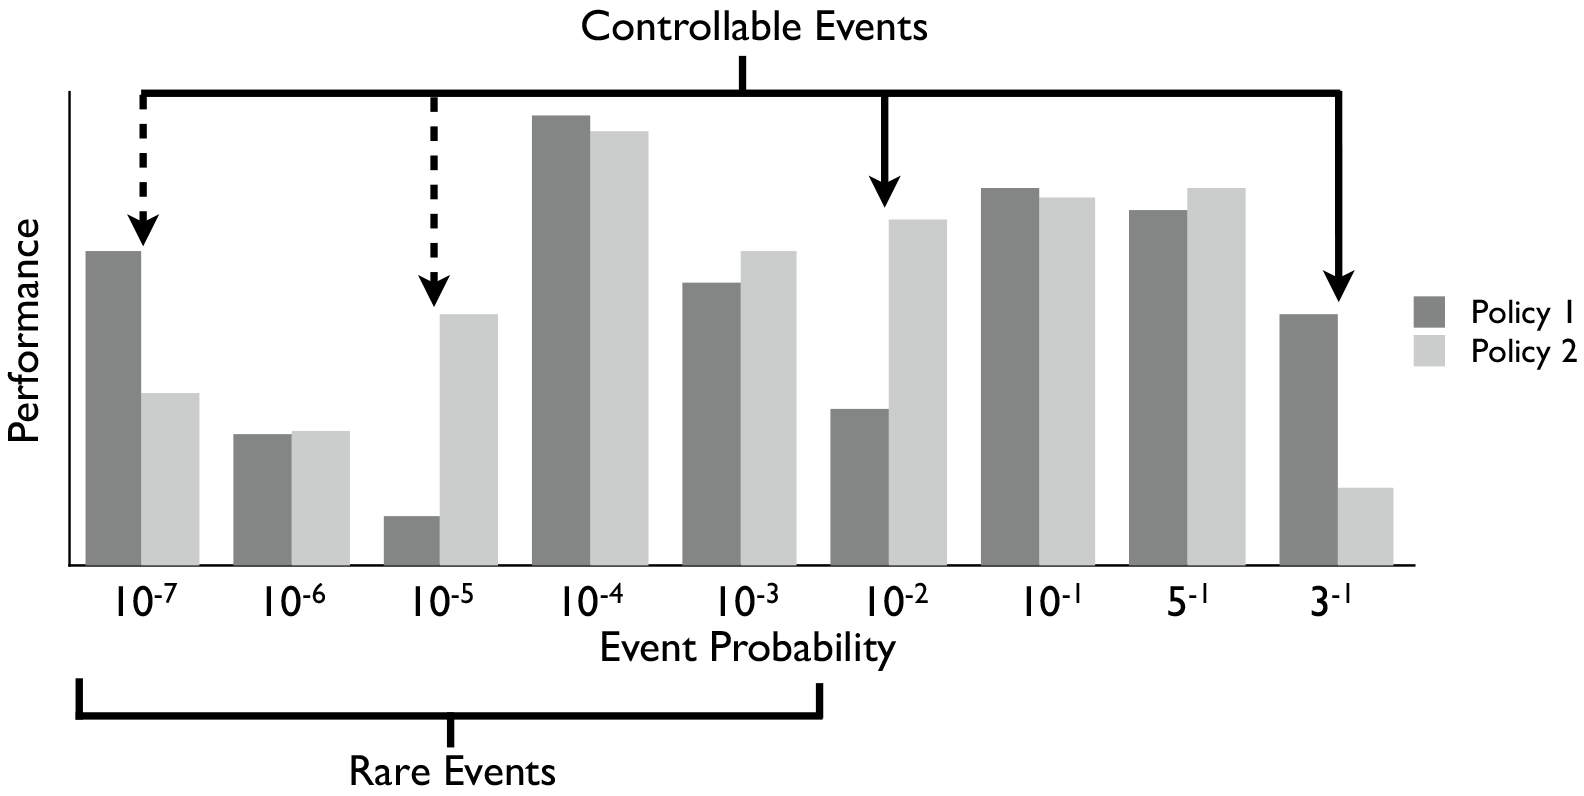
\includegraphics{images/rare-controllable.png}
%   \caption{Performance of two policies on a set of events, showing rare-, controllable- and rare controllable events}\label{rareControllableImage}
% \end{figure}

Controllable events are interesting because they are important to learn (as learning the correct policy in such an event is rewarding). Additionally, as rare events do not occur often, general reinforcement learning often does not consider them and thus the agent does not learn how to act in such a situation. As a direct consequence of the nature of rare controllable events, an agent often does not know how to act optimally in such events, while acting sub-optimal could result in a significantly lower reward.

\subsection{Neural Networks}
% meer in detail propagation uitleggen?
Neural networks are inspired by the central nervous systems and describe a set of nodes of which the (one-directional) connection contain weights. Nodes can be of three types: input-, output- or hidden nodes. The input nodes receive a signal (value), which are propagated to the next layer of nodes by multiplication with the corresponding weights. The values are propagated through the network and eventually reach the output nodes, which defines the output of the network. 

In the current setting, networks are used as policies. The current situation (state) is the input, whereas the output of the network is the action to take. 

\subsection{Gaussian Process}
% TODO

\subsection{(Co) evolution}
% TODO
In the process of creating a better believe of the fitness over the policies, a method is required to define new policies. 


% outro
In the following section (\ref{related}) the related work will be described, followed by our contribution (\ref{contrib}). We then describe the experiments (\ref{experiments}), discuss them and lastly conclude (\ref{conclusion}).

